\documentclass{beamer}
%
% Choose how your presentation looks.
%
% For more themes, color themes and font themes, see:
% http://deic.uab.es/~iblanes/beamer_gallery/index_by_theme.html
%
\mode<presentation>
{
  \usetheme{Madrid}      % or try Darmstadt, Madrid, Warsaw, ...
  \usecolortheme{seahorse} % or try albatross, beaver, crane, ...
  \usefonttheme{serif}  % or try serif, structurebold, ...
  \setbeamertemplate{navigation symbols}{}
  \setbeamertemplate{caption}[numbered]
} 

\usepackage[english]{babel}
\usepackage{kotex}
\usepackage{tikz}
\usepackage{listings}
\usepackage{pgffor}
\input{algorithmbisEnv.tex}

\title[3D 그래픽스 프로그래밍]{그래픽스 강의노트 03 - OpenGL 소개}
\author{강영민}
\institute{동명대학교}
\date{2016년 2학기}

\begin{document}

%%%%%%%%%%%%%%%%%%%%%%%%%%%%%%%%%%%%%%%%%%%%%%%%%%%%%%%%%
\begin{frame}
  \titlepage
\end{frame}

% Uncomment these lines for an automatically generated outline.
%\begin{frame}{Outline}
%  \tableofcontents
%\end{frame}


%%%%%%%%%%%%%%%%%%%%%%%%%%%%%%%%%%%%%%%%%%%%%%%%%%%%%%%%%
\begin{frame}{OpenGL}

\begin{itemize}
\item OpenGL은 특정한 하드웨어나 운영체제에 의존하지 않고 다양한 시스템에 이식(移植)될 수 있는 개방형 라이브러리
\item OpenGL을 통한 학습은 실시간 그래픽스에 대한 이해를 돕고, 다양한 시스템에 적용가능한 그래픽스 프로그래밍 기술을 습득하게 함
\end{itemize}
\end{frame}
%%%%%%%%%%%%%%%%%%%%%%%%%%%%%%%%%%%%%%%%%%%%%%%%%%%%%%%%%

%%%%%%%%%%%%%%%%%%%%%%%%%%%%%%%%%%%%%%%%%%%%%%%%%%%%%%%%%
\begin{frame}{OpenGL을 사용하기 위한 준비}

\begin{itemize}
\item Mac OS X, Linux - 특별한 준비가 필요 없음
\item MS Windows - 플랫폼 독립적 윈도우 생성을 위해 glut를 따로 설치해야 함
\end{itemize}


\begin{itemize}
\item 수업에 사용할 glut 라이브러리
	\begin{itemize}
	\item freeglut
	\item 다운로드 - precompiled binary는 64비트 
	\item 32비트와 64비트 용으로 컴파일한 결과를 수업 홈페이지에 게시
	\end{itemize}
\end{itemize}

\end{frame}
%%%%%%%%%%%%%%%%%%%%%%%%%%%%%%%%%%%%%%%%%%%%%%%%%%%%%%%%%


%%%%%%%%%%%%%%%%%%%%%%%%%%%%%%%%%%%%%%%%%%%%%%%%%%%%%%%%%
\begin{frame}{MS Windows 환경에서 freeglut 설치}

\begin{itemize}
\item 32비트
	\begin{itemize}
	\item freeglutd.dll, freeglut.dll $\rightarrow$ C:$\backslash$Windows$\backslash$System32
	\item 헤더 파일들 $\rightarrow$ (Windows SDK)$\backslash$include$\backslash$GL
	\item 라이브러리 파일들 (freeglutd.lib, freeglut.lib) $\rightarrow$ (Windows SDK)$\backslash$lib
	\end{itemize}
\end{itemize}

\begin{itemize}
\item 64비트
	\begin{itemize}
	\item freeglutd.dll, freeglut.dll $\rightarrow$ C:$\backslash$Windows$\backslash$SystemWOW64
	\item 헤더 파일들 $\rightarrow$ (Windows SDK)$\backslash$include$\backslash$GL
	\item 라이브러리 파일들 (freeglutd.lib, freeglut.lib) $\rightarrow$ (Windows SDK)$\backslash$lib$\backslash$x64
	\end{itemize}
\item 프로젝트의 플랫폼을 Win32가 아니라 64비트로 변경하여 생성하여야 함
\end{itemize}

\end{frame}
%%%%%%%%%%%%%%%%%%%%%%%%%%%%%%%%%%%%%%%%%%%%%%%%%%%%%%%%%


%%%%%%%%%%%%%%%%%%%%%%%%%%%%%%%%%%%%%%%%%%%%%%%%%%%%%%%%%
\begin{frame}[fragile]{간단한 OpenGL 프로그램 테스트}
\lstset{language=C++,escapechar=^} 
\begin{lstlisting}
#include "headers.h"

void myDisplay() {
    glClear(GL_COLOR_BUFFER_BIT);
    glFlush();    
}
int main (int argc, char * argv[]) {
    glutInit(&argc, argv);
    glutInitDisplayMode(GLUT_SINGLE|GLUT_RGBA);
    glutInitWindowPosition(0, 0);
    glutInitWindowSize(512, 512);
    glutCreateWindow("A Triangle");  // ^{\it 윈도우 생성}^

    glClearColor(1.0, 0.0, 0.0, 1.0);
    glutDisplayFunc(myDisplay);	// ^{\it 디스플레이 콜백 등록}^
    glutMainLoop();				// ^{\it 이벤트 루프}^
    return 0;
}
\end{lstlisting}
\end{frame}
%%%%%%%%%%%%%%%%%%%%%%%%%%%%%%%%%%%%%%%%%%%%%%%%%%%%%%%%%

%%%%%%%%%%%%%%%%%%%%%%%%%%%%%%%%%%%%%%%%%%%%%%%%%%%%%%%%%
\begin{frame}{OpenGL의 특징}

\begin{itemize}
\item 실시간 그래픽 라이브러리로서 사실상의 ({\it de facto}) 산업 표준
\item 플랫폼에 독립적
	\begin{itemize}
	\item OpenGL을 이용하여 작성한 그래픽 프로그램은 여러 종류의 다른 운영체제를 가진 시스템에 쉽게 이식
	\end{itemize}
\item OpenGL은 상태 기계(state machine)
	\begin{itemize}
	\item OpenGL의 동작은 현재의 상태에 의해 결정
	\item 이 상태는 변경하지 않으면 계속해서 유지
	\item OpenGL에는 많은 종류의 상태 변수가 있으며, 이 상태는 한 번 설정하면 다시 변경하지 않는 한 계속해서 설정된 상태를 유지
	\item 예: 선의 두께를 결정했다면, 이후에 이 두께를 변경하지 않는 이상 모든 선이 설정된 두께로 그려짐	
	\end{itemize}
\end{itemize}

\end{frame}
%%%%%%%%%%%%%%%%%%%%%%%%%%%%%%%%%%%%%%%%%%%%%%%%%%%%%%%%%

%%%%%%%%%%%%%%%%%%%%%%%%%%%%%%%%%%%%%%%%%%%%%%%%%%%%%%%%%
\begin{frame}{OpenGL의 관례}

\begin{itemize}
\item OpenGL API의 명령들은 gl-Command-dimension-type의 꼴
	\begin{itemize}
	\item glVertex3f는 정점(Vertex)의 위치를 설정하는 OpenGL 명령으로 3차원 데이터이며, 각 차원의 값을 부동소수점(floating point)로 표현한다는 의미
	\end{itemize}
\item OpenGL 명령어의 뒤에 붙어 입력 파라미터의 자료형을 표시하는 접미사는 표와 같음
\end{itemize}

\begin{table}
\begin{tabular}{|c|l|l|l|} \hline
f & 32 비트 부동소수점 & float & GLfloat \\ \hline
d & 64 비트 부동소수점 & double & GLdouble \\ \hline
b & 8 비트 정수 & char & GLbyte \\ \hline
ub & 8 비트 부호 없는 정수 & unsigned char & GLubyte \\ \hline
i & 32 비트 정수 & int or long & GLint \\ \hline
ui & 32 비트 부호 없는 정수  & unsigned int$|$long & GLuint, GLenum \\ \hline
s & 16 비트 정수 & short & GLshort \\ \hline
\end{tabular}
\end{table}

\end{frame}
%%%%%%%%%%%%%%%%%%%%%%%%%%%%%%%%%%%%%%%%%%%%%%%%%%%%%%%%%


%%%%%%%%%%%%%%%%%%%%%%%%%%%%%%%%%%%%%%%%%%%%%%%%%%%%%%%%%
\begin{frame}{OpenGL의 관례}

{\small 
\begin{itemize}
\item OpenGL API의 명령들은 gl-Command-dimension-type의 꼴
	\begin{itemize}
	\item glVertex3f는 정점(Vertex)의 위치를 설정하는 OpenGL 명령으로 3차원 데이터이며, 각 차원의 값을 부동소수점으로 표현한다는 의미
	\end{itemize}
\item 입력 파라미터의 자료형을 표시하는 접미사는 표와 같음
\end{itemize}

\begin{table}
\begin{tabular}{|c|l|l|l|} \hline
f & 32 비트 부동소수점 & float & GLfloat \\ \hline
d & 64 비트 부동소수점 & double & GLdouble \\ \hline
b & 8 비트 정수 & char & GLbyte \\ \hline
ub & 8 비트 부호 없는 정수 & unsigned char & GLubyte \\ \hline
i & 32 비트 정수 & int or long & GLint \\ \hline
ui & 32 비트 부호 없는 정수  & unsigned int$|$long & GLuint, GLenum \\ \hline
s & 16 비트 정수 & short & GLshort \\ \hline
\end{tabular}
\end{table}
}
\begin{block}{GLU(GL Utility)와 GLUT(GL Utility Toolkit)}
{\small 카메라 등을 다루는 OpenGL 유틸리티 라이브러리의 명령들은 glu로 시작한다. 또한 서로 다른 윈도 환경에 독립적인 윈도 관리를 지원하는 OpenGL 유틸리티 툴킷 (utility toolkit)을 사용하는데, 이 툴킷의 명령들은 glut로 시작한다.}
\end{block}

\end{frame}
%%%%%%%%%%%%%%%%%%%%%%%%%%%%%%%%%%%%%%%%%%%%%%%%%%%%%%%%%


%%%%%%%%%%%%%%%%%%%%%%%%%%%%%%%%%%%%%%%%%%%%%%%%%%%%%%%%%
\begin{frame}[fragile]{OpenGL 프로그램의 기본 형태}
\lstset{language=C++,escapechar=^} 
\begin{lstlisting}
#include ^{\it whatever you want}^
callback_for_display() {
   for(^{\sf 그려질 모든 객체에 대해^) {
      ^{\it 변환 설정;}^
      glBegin(^{\sf 그리기 프리미티브 지정}^);
      	^{\sf [[정점(vertex) 정보 제공;]]}^
      glEnd(); 
   }
   glFlush() ^{\it 또는}^ glutSwapBuffers();
}
void main(int argc, char **argv) {
   ^{\sf [[윈도우 초기화;]]}^
   glMatrixMode(GL_PROJECTION); 
   ^{\sf [[투영 행렬 설정;]]}^
   glMatrixMode(GL_MODELVIEW); 
   ^{\sf [[카메라의 위치와 방향 잡기;]]}^
   ^{\sf [[콜백 함수의 등록;]]}^
   ^{\sf [[메인 루프로 들어가기;]]}^
}
\end{lstlisting}
\end{frame}


%%%%%%%%%%%%%%%%%%%%%%%%%%%%%%%%%%%%%%%%%%%%%%%%%%%%%%%%%
\begin{frame}{간단한 OpenGL 프로그램의 예}
    \lstset{language=C++,frame=none,escapechar=^}%
    \foreach \n in {1,26,...,50} {%
       \only<+>{%
            \edef\m{\the\numexpr\n+24\relax}%
            \edef\thesubtitle{{Lines \n--\m\ / 50}}%
            \expandafter\framesubtitle\thesubtitle
            \lstinputlisting[firstline=\n,lastline=\m]{./Codes/L03_simpleGL.tex}%
       }%
    }
\end{frame}

%%%%%%%%%%%%%%%%%%%%%%%%%%%%%%%%%%%%%%%%%%%%%%%%%%%%%%%%%

%%%%%%%%%%%%%%%%%%%%%%%%%%%%%%%%%%%%%%%%%%%%%%%%%%%%%%%%%


\begin{frame}{간단한 OpenGL 프로그램의 예}

\begin{figure}
    \includegraphics[height=6cm]{OGL_opengl/simpleEx.png}
\end{figure}

\end{frame}

%%%%%%%%%%%%%%%%%%%%%%%%%%%%%%%%%%%%%%%%%%%%%%%%%%%%%%%%%

%%%%%%%%%%%%%%%%%%%%%%%%%%%%%%%%%%%%%%%%%%%%%%%%%%%%%%%%%
\begin{frame}[fragile]{프리미티브(primitives) - 1/3}

\begin{itemize}
\item 그래픽 하드웨어는 프로그래머(programmer)가 지정한 프리미티브(primitive) 설정에 따라 정점의 리스트를 처리
\item 프리미티브는 OpenGL이 제공하는 그리기 기본요소
\item 입력 정점들을 어떻게 조합할 것인가를 결정
\end{itemize}

\begin{itemize}
\item 프리미티브를 사용하는 방법은 다음과 같다.
\end{itemize}

\lstset{language=C++,escapechar=^} 
\begin{lstlisting}
glBegin(^{\sf drawing primitive}^);
      // vertex position, color, normal, etc
      setVertexInfo(); 
glEnd(); 
}

\end{lstlisting}

\end{frame}
%%%%%%%%%%%%%%%%%%%%%%%%%%%%%%%%%%%%%%%%%%%%%%%%%%%%%%%%%

%%%%%%%%%%%%%%%%%%%%%%%%%%%%%%%%%%%%%%%%%%%%%%%%%%%%%%%%%
\begin{frame}[fragile]{프리미티브(primitives) - 2/3}

{\small
\begin{itemize}
\item {\sf GL\_POINTS}: 입력된 정점을 하나씩 점으로 가시화
\item {\sf GL\_LINES}: 입력된 정점을 두 개씩 묶어 선분으로 표현 
\item {\sf GL\_LINE\_STRIP}: 입력된 정점을 차례대로 연결하여 하나의 폴리라인(polyline)을 구성
\item {\sf GL\_LINE\_LOOP}: 입력된 정점을 차례로 연결한 뒤에 마지막 점을 시작점으로 연결
\item {\sf GL\_TRIANGLES}: 입력된 정점을 세 개씩 묶어 삼각형을 그림
\item {\sf GL\_TRIANGLE\_STRIP}: 처음 세 개 정점으로 삼각형을 그린 뒤, 정점이 추가될 때마다 삼각형을 직전 두 개 정점과 연결하여 삼각형 추가 
\item {\sf GL\_TRIANGLE\_FAN}: 부채 모양으로 삼각형을 추가해 나감
\item {\sf GL\_QUADS}: 정점 네 개씩을 묶어 사각형 그리기
\item {\sf GL\_QUAD\_STRIP}: 처음 네 개 정점으로 사각형 그리고, 이후 두 개씩 묵어 직전 두 개 정점과 함께 사각형 그리기
\item {\sf GL\_POLYGON}: 입력된 모든 정점으로 다각형을 그림
\end{itemize}
}


\end{frame}
%%%%%%%%%%%%%%%%%%%%%%%%%%%%%%%%%%%%%%%%%%%%%%%%%%%%%%%%%


%%%%%%%%%%%%%%%%%%%%%%%%%%%%%%%%%%%%%%%%%%%%%%%%%%%%%%%%%
\begin{frame}[fragile]{프리미티브(primitives) - 3/3}

\begin{figure}
\includegraphics[height=6cm]{OGL_opengl/primitives.png}
\end{figure}


\end{frame}
%%%%%%%%%%%%%%%%%%%%%%%%%%%%%%%%%%%%%%%%%%%%%%%%%%%%%%%%%


%%%%%%%%%%%%%%%%%%%%%%%%%%%%%%%%%%%%%%%%%%%%%%%%%%%%%%%%%
\begin{frame}[fragile]{정점 데이터 설정 방법}

\begin{itemize}
\item 정점 데이터는 위치와 법선벡터, 색 등
\item 정점의 위치만을 입력한다면 glVertex[dim-type]으로 입력
\item 3 차원 정점의 각 성분을 부동소수점 표현으로 넣는다면, glVertex3f(x,y,z)와 같이 입력
\item 다음과 같은 같은 여러 표현이 가능하다.
\end{itemize}

\lstset{language=C++} 
\begin{lstlisting}
float x,y,z;
double dx,dy,dz;
int ix,iy,iz;
float verts = {1.0f, 2.0f, 1.0f};
glBegin(drawing primitive);
      glVertex3f(x,y,z);
      glVertex3d(dx,dy,dz);
      glVertex3i(ix,iy,iz);
      glVertex3fv(verts);
glEnd();
\end{lstlisting}

\end{frame}
%%%%%%%%%%%%%%%%%%%%%%%%%%%%%%%%%%%%%%%%%%%%%%%%%%%%%%%%%

%%%%%%%%%%%%%%%%%%%%%%%%%%%%%%%%%%%%%%%%%%%%%%%%%%%%%%%%%
\begin{frame}[fragile]{다양한 프리미티브를 이용한 풍경 그리기}

    \lstset{language=C++,frame=none,escapechar=^}%
    \foreach \n in {1,26,...,75} {%
       \only<+>{%
            \edef\m{\the\numexpr\n+24\relax}%
            \edef\thesubtitle{{Lines \n--\m\ / 75}}%
            \expandafter\framesubtitle\thesubtitle
            \lstinputlisting[firstline=\n,lastline=\m]{./Codes/L03_sceneWithPrimitives.tex}%
       }%
    }

\end{frame}
%%%%%%%%%%%%%%%%%%%%%%%%%%%%%%%%%%%%%%%%%%%%%%%%%%%%%%%%%

%%%%%%%%%%%%%%%%%%%%%%%%%%%%%%%%%%%%%%%%%%%%%%%%%%%%%%%%%
\begin{frame}[fragile]{다양한 프리미티브를 이용한 풍경 그리기}

\begin{figure}
    \includegraphics[height=7cm]{OGL_opengl/simpleScene.png}
\end{figure}


\end{frame}
%%%%%%%%%%%%%%%%%%%%%%%%%%%%%%%%%%%%%%%%%%%%%%%%%%%%%%%%%

%%%%%%%%%%%%%%%%%%%%%%%%%%%%%%%%%%%%%%%%%%%%%%%%%%%%%%%%%
\begin{frame}[fragile]{디폴트 카메라}

\begin{itemize}
\item OpenGL의 디폴트 카메라는 원점 위치
\item z축 음의 방향
\item 원근 투영을 적용하지 않아 카메라에 잡히는 공간은 상자 형태
\end{itemize}

\begin{figure}
    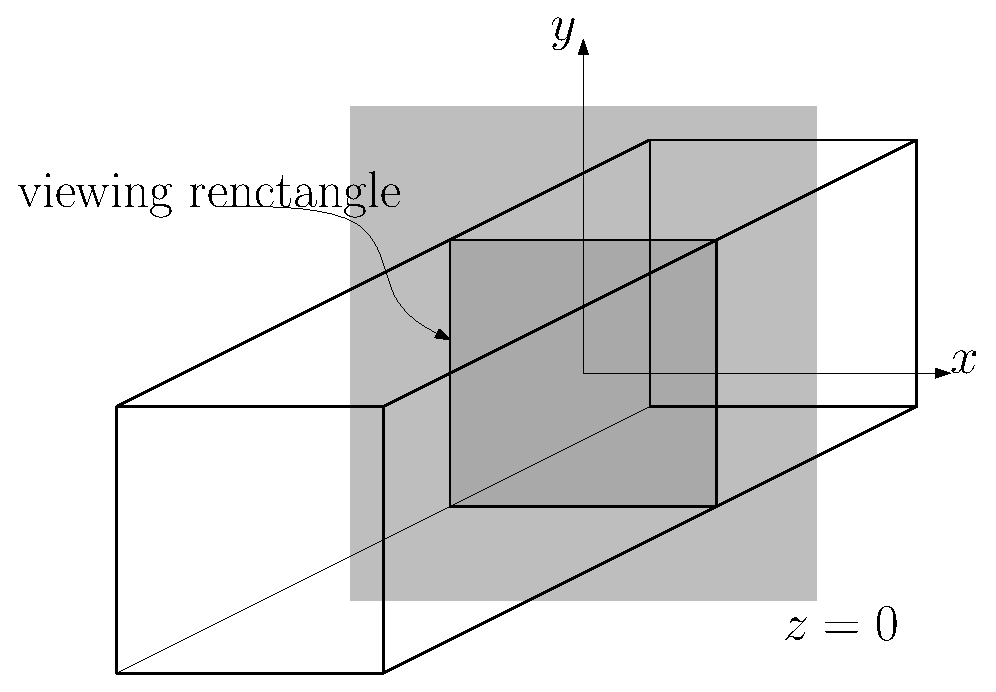
\includegraphics[height=5cm]{OGL_opengl/defaultCam.eps}
\end{figure}


\end{frame}
%%%%%%%%%%%%%%%%%%%%%%%%%%%%%%%%%%%%%%%%%%%%%%%%%%%%%%%%%

%%%%%%%%%%%%%%%%%%%%%%%%%%%%%%%%%%%%%%%%%%%%%%%%%%%%%%%%%
\begin{frame}[fragile]{직교 투영 (orthographics projection) 설정}

\begin{itemize}
\item 디폴트 카메라는 직교 투영 카메라
\item 상자 모양의 가시화 공간내의 객체를 상자를 절단하는 면에 투영
\item 이 상자의 위치와 길이를 변경하는 함수가 glOrtho
\end{itemize}

\begin{figure}
    \includegraphics[height=4cm]{OGL_opengl/glOrtho.eps}
\end{figure}
\begin{center}{\tiny glOrtho(float left, float right, float bottom, float top, float near, float far);}
\end{center}

\begin{itemize}
\item 결국 OpenGL의 디폴트 카메라는 다음과 같은 설정
	\begin{itemize}
	\item glOrtho(-1,1, -1,1, -1,1);
	\end{itemize}
\end{itemize}

\end{frame}
%%%%%%%%%%%%%%%%%%%%%%%%%%%%%%%%%%%%%%%%%%%%%%%%%%%%%%%%%

%%%%%%%%%%%%%%%%%%%%%%%%%%%%%%%%%%%%%%%%%%%%%%%%%%%%%%%%%
\begin{frame}[fragile]{원근 투영 (perspective projection) 설정}

{\small
\begin{itemize}
\item 실제 카메라나 우리 눈은 원근이 없는 평행 투영이 불가능
\item 멀리 있는 것은 작게 보이고 가까이 있는 것은 크게 보이는 이유는 원근투영
\item 이러한 원근 투영을 설정하는 방법은 {\sf glFrustum}과 {\sf gluPerspective}
\item {\sf glFrustum}에 대한 이해는 뒤로 미루고 우선 직관적인 {\sf  gluPerspective} 함수를 먼저 이해
\end{itemize}

\begin{verbatim}
gluPerspective(float fovy, float Aspect, float near, float far);
\end{verbatim}


\begin{itemize}
\item {\sf fovy}는 $y$축 방향으로의 시야각을 도(degree)로 나타낸 것
\item {\sf Aspect}는 가시화 볼륨의 종횡비(aspect ratio)
\item {\sf near}는 카메라에서 상이 맺히는 가까운 평면까지의 거리
\item {\sf far}는 가시화 공간을 결정하는 평면 중 카메라에서 가장 먼 쪽 평면과 카메라 사이의 거리
\item 이 함수는 그리기 동작이 일어날 때마다 불리는 것이 아니라 초기에 한 번, 혹은 렌즈를 바꿀 필요가 있을 때에만 불린다.
\end{itemize}
}

\end{frame}
%%%%%%%%%%%%%%%%%%%%%%%%%%%%%%%%%%%%%%%%%%%%%%%%%%%%%%%%%

%%%%%%%%%%%%%%%%%%%%%%%%%%%%%%%%%%%%%%%%%%%%%%%%%%%%%%%%%
\begin{frame}[fragile]{행렬 모드(matrix mode)}

{\small
\begin{itemize}
\item OpenGL은 세 종류의 행렬: 텍스처 행렬, 모델뷰 행렬, 투영행렬
\item 모델뷰 행렬은 공간 내에서 가상 객체의 좌표를 변경
\item 투영행렬은 가상 객체를 투영면에 옮겨 놓음
\end{itemize}

\lstset{language=C++, escapechar=^} 
\begin{lstlisting}
glMatrixMode(GL_PROJECTION);
glLoadIdentity();
gluPerspective(60, 1.0, 0.1, 100.0);

glMatrixMode(GL_MODELVIEW);
glLoadIdentity();
gluLookAt(1.0, 1.0, 1.0, 0.0, 0.0, 0.0, 0.0, 1.0, 0.0);

^{\sf [[draw something]]}^
\end{lstlisting}

\begin{itemize}
\item 여기서는 {\sf gluPerspective}와 {\sf gluLookAt}이 어떠한 행렬 모드을 변경하는가 하는 것이 관심
\item {\sf gluPerspective} 함수는 투영의 특성을 변경하는 것이므로 투영행렬 모드
\item {\sf gluLookAt}은 카메라의 위치를 옮기는 것이고, 이는 바꾸어 말해 물체의 위치를 카메라 기준에서 옮기는 것이므로 모델뷰 행렬을 변경
\end{itemize}
}

\end{frame}
%%%%%%%%%%%%%%%%%%%%%%%%%%%%%%%%%%%%%%%%%%%%%%%%%%%%%%%%%

%%%%%%%%%%%%%%%%%%%%%%%%%%%%%%%%%%%%%%%%%%%%%%%%%%%%%%%%%
\begin{frame}[fragile]{카메라 위치 변경}

\begin{itemize}
\item 카메라를 원하는 곳으로 옮겨주는 함수:  {\sf gluLookAt}
\end{itemize}


\begin{verbatim}
gluLookAt(float eye_x, float eye_y, float eye_z,
          float at_x, float at_y, float at_z,
          float up_x, float up_y, float up_z);
\end{verbatim}


\begin{itemize}
\item 카메라의 위치를 옮겨 놓는 역학
\item 카메라 이동의 반대로 물체를 옮겨 놓는 것
\item 카메라의 위치는 매 프레임마다 변경될 수 있으므로 이 함수는 그리기 함수 내에서 매번 불리는 것이 일반적
\end{itemize}

\end{frame}
%%%%%%%%%%%%%%%%%%%%%%%%%%%%%%%%%%%%%%%%%%%%%%%%%%%%%%%%%

%%%%%%%%%%%%%%%%%%%%%%%%%%%%%%%%%%%%%%%%%%%%%%%%%%%%%%%%%
\begin{frame}[fragile]{카메라를 설정하는 기본적인 프로그램}

    \lstset{language=C++,frame=none,escapechar=^}%
    \foreach \n in {1,26,...,50} {%
       \only<+>{%
            \edef\m{\the\numexpr\n+24\relax}%
            \edef\thesubtitle{{Lines \n--\m\ / 50}}%
            \expandafter\framesubtitle\thesubtitle
            \lstinputlisting[firstline=\n,lastline=\m]{./Codes/L03_simpleCamera.tex}%
       }%
    }

\end{frame}
%%%%%%%%%%%%%%%%%%%%%%%%%%%%%%%%%%%%%%%%%%%%%%%%%%%%%%%%%


%%%%%%%%%%%%%%%%%%%%%%%%%%%%%%%%%%%%%%%%%%%%%%%%%%%%%%%%%
\begin{frame}[fragile]{카메라 조작 결과}

\begin{figure}
    \includegraphics[height=7cm]{OGL_opengl/camMove.png}
\end{figure}

\end{frame}
%%%%%%%%%%%%%%%%%%%%%%%%%%%%%%%%%%%%%%%%%%%%%%%%%%%%%%%%%

%%%%%%%%%%%%%%%%%%%%%%%%%%%%%%%%%%%%%%%%%%%%%%%%%%%%%%%%%
\begin{frame}[fragile]{카메라 조작 결과}

\begin{figure}
    \includegraphics[height=7cm]{OGL_opengl/camMove.png}
\end{figure}

\end{frame}
%%%%%%%%%%%%%%%%%%%%%%%%%%%%%%%%%%%%%%%%%%%%%%%%%%%%%%%%%


%%%%%%%%%%%%%%%%%%%%%%%%%%%%%%%%%%%%%%%%%%%%%%%%%%%%%%%%%
\begin{frame}[fragile]{(깊이버퍼 없이) 네 개의 면으로 상자 모양 그리기}

    \lstset{language=C++,frame=none,escapechar=^}%
    \foreach \n in {1,26,...,50} {%
       \only<+>{%
            \edef\m{\the\numexpr\n+24\relax}%
            \edef\thesubtitle{{Lines \n--\m\ / 50}}%
            \expandafter\framesubtitle\thesubtitle
            \lstinputlisting[firstline=\n,lastline=\m]{./Codes/L03_simple3D.tex}%
       }%
    }

\end{frame}
%%%%%%%%%%%%%%%%%%%%%%%%%%%%%%%%%%%%%%%%%%%%%%%%%%%%%%%%%


%%%%%%%%%%%%%%%%%%%%%%%%%%%%%%%%%%%%%%%%%%%%%%%%%%%%%%%%%
\begin{frame}[fragile]{(깊이버퍼 없이) 네 개의 면으로 상자 모양 그리기}
\begin{figure}
    \includegraphics[height=7cm]{OGL_opengl/noZBuff.png}
\end{figure}
\end{frame}
%%%%%%%%%%%%%%%%%%%%%%%%%%%%%%%%%%%%%%%%%%%%%%%%%%%%%%%%%


%%%%%%%%%%%%%%%%%%%%%%%%%%%%%%%%%%%%%%%%%%%%%%%%%%%%%%%%%
\begin{frame}[fragile]{깊이 버퍼 (depth buffer)}

{\small
\begin{figure}
\begin{tabular}{p{6.5cm}c}
\begin{itemize}
\item 깊이 버퍼 혹은 z-버퍼
	\begin{itemize}
	\item 색상 버퍼(color buffer)는 그려지는 영상의 각 화소별 색을 기록
	\item 우리가 최종적으로 보게되는 것은 이 색상 버퍼의 내용
	\item 색상 버퍼를 구성할 때 물체의 가려짐을 고려하여 가려진 물체를 그리지 않도록 하는 버퍼가 깊이 버퍼
	\item 색상이 아니라 카메라에서 그려지는 픽셀까지의 거리를 저장하는 버퍼
	\end{itemize}
\end{itemize}
&
\raisebox{-\totalheight}{\includegraphics[height=6cm]{OGL_opengl/Z_Buffer.png}}
\end{tabular}
\end{figure}
}

\end{frame}
%%%%%%%%%%%%%%%%%%%%%%%%%%%%%%%%%%%%%%%%%%%%%%%%%%%%%%%%%


%%%%%%%%%%%%%%%%%%%%%%%%%%%%%%%%%%%%%%%%%%%%%%%%%%%%%%%%%
\begin{frame}[fragile]{깊이 버퍼의 사용}

{\small
\begin{itemize}
\item OpenGL에서는 이러한 깊이 버퍼를 쉽게 사용할 수 있도록 지원
	\begin{itemize}
	\item{\sf glutInitDisplayMode(GLUT\_SINGLE $|$ \color{red}{GLUT\_DEPTH} $|$ GLUT\_RGBA);}
	\end{itemize}
\end{itemize}

\begin{itemize}
\item 기본적으로 “깊이 테스트” 작업을 수행하지 않는 것이 디폴트
\item 깊이 테스트를 수행하기 위해서는 다음과 같이 상태를 변경
	\begin{itemize}
	\item{\sf glEnable(\color{red}{GL\_DEPTH\_TEST});}
	\end{itemize}
\end{itemize}



\begin{itemize}
\item 또한 매번 그리기가 이뤄지면 그려진 내용에 따라 깊이 버퍼의 내용이 더러워져 있는 상태
\item 새로운 그리기를 하기 전에 색상 버퍼를 깨끗하게 지우듯이 깊이 버퍼의 내용도 깨끗하게 지우는 다음과 같은 코드가 필요
	\begin{itemize}
	\item{\sf glClear( GL\_COLOR\_BUFFER\_BIT $|$ \color{red}{GL\_DEPTH\_BUFFER\_BIT});}
	\end{itemize}
\end{itemize}
}


\end{frame}
%%%%%%%%%%%%%%%%%%%%%%%%%%%%%%%%%%%%%%%%%%%%%%%%%%%%%%%%%


%%%%%%%%%%%%%%%%%%%%%%%%%%%%%%%%%%%%%%%%%%%%%%%%%%%%%%%%%
\begin{frame}[fragile]{깊이 버퍼와 이중 버퍼 사용 예제}

{\small
\begin{itemize}
\item 지금까지 색상과 깊이 버퍼가 하나만 존재하는 단일 버퍼 환경
\item 단일 버퍼 환경은 애니메이션 등이 있을 때 깜빡임 발생 가능
\item 해결: 앞 버퍼(front buffer)와 뒷 버퍼(back buffer)의 이중 구조
	\begin{itemize}
	\item {\sf glutInitDisplayMode({\color{red}GLUT\_DOUBLE$|$GLUT\_DEPTH$|$GLUT\_RGBA});}
	\end{itemize}
\item 디스플레이 장치로 프레임 버퍼를 보내는 것은 {\sf glFlush}가 아니라 {\sf glutSwapBuffers}를 이용
	\begin{itemize}
	\item {\sf glutSwapBuffers();}
	\end{itemize}
\end{itemize}

}


\end{frame}
%%%%%%%%%%%%%%%%%%%%%%%%%%%%%%%%%%%%%%%%%%%%%%%%%%%%%%%%%

%%%%%%%%%%%%%%%%%%%%%%%%%%%%%%%%%%%%%%%%%%%%%%%%%%%%%%%%%
\begin{frame}[fragile]{깊이 버퍼와 이중 버퍼 사용 예제}
    \lstset{language=C++,frame=none,escapechar=^}%
    \foreach \n in {1,26,...,50} {%
       \only<+>{%
            \edef\m{\the\numexpr\n+24\relax}%
            \edef\thesubtitle{{Lines \n--\m\ / 50}}%
            \expandafter\framesubtitle\thesubtitle
            \lstinputlisting[firstline=\n,lastline=\m]{./Codes/L03_depthAndDoubleBuffers.tex}%
       }%
    }
\end{frame}
%%%%%%%%%%%%%%%%%%%%%%%%%%%%%%%%%%%%%%%%%%%%%%%%%%%%%%%%%

%%%%%%%%%%%%%%%%%%%%%%%%%%%%%%%%%%%%%%%%%%%%%%%%%%%%%%%%%
\begin{frame}[fragile]{깊이 버퍼와 이중 버퍼 사용 결과}

\begin{figure}
    \includegraphics[height=7cm]{OGL_opengl/ZBuff.png}
\end{figure}

\end{frame}
%%%%%%%%%%%%%%%%%%%%%%%%%%%%%%%%%%%%%%%%%%%%%%%%%%%%%%%%%

\end{document}



